% 若编译失败,且生成 .synctex(busy) 辅助文件,可能有两个原因:
% 1. 需要插入的图片不存在:Ctrl + F 搜索 'figure' 将这些代码注释/删除掉即可
% 2. 路径/文件名含中文或空格:更改路径/文件名即可

% ------------------------------------------------------------- %
% >> ------------------ 文章宏包及相关设置 ------------------ << %
% 设定文章类型与编码格式
\documentclass[UTF8]{report}		

% 本文特殊宏包
\usepackage{siunitx} % 埃米单位

% 本 .tex 专属的宏定义
    \def\V{\ \mathrm{V}}
    \def\mV{\ \mathrm{mV}}
    \def\kV{\ \mathrm{KV}}
    \def\KV{\ \mathrm{KV}}
    \def\MV{\ \mathrm{MV}}
    \def\A{\ \mathrm{A}}
    \def\mA{\ \mathrm{mA}}
    \def\kA{\ \mathrm{KA}}
    \def\KA{\ \mathrm{KA}}
    \def\MA{\ \mathrm{MA}}
    \def\O{\ \Omega}
    \def\mO{\ \Omega}
    \def\kO{\ \mathrm{K}\Omega}
    \def\KO{\ \mathrm{K}\Omega}
    \def\MO{\ \mathrm{M}\Omega}
    \def\Hz{\ \mathrm{Hz}}

% 自定义宏定义
    \def\N{\mathbb{N}}
    \def\F{\mathbb{F}}
    \def\Z{\mathbb{Z}}
    \def\Q{\mathbb{Q}}
    \def\R{\mathbb{R}}
    \def\C{\mathbb{C}}
    \def\T{\mathbb{T}}
    \def\S{\mathbb{S}}
    \def\A{\mathbb{A}}
    \def\I{\mathscr{I}}
    \def\Im{\mathrm{Im\,}}
    \def\Re{\mathrm{Re\,}}
    \def\d{\mathrm{d}}
    \def\p{\partial}

% 导入基本宏包
    \usepackage[UTF8]{ctex}     % 设置文档为中文语言
    \usepackage[colorlinks, linkcolor=blue, anchorcolor=blue, citecolor=blue, urlcolor=blue]{hyperref}  % 宏包:自动生成超链接 (此宏包与标题中的数学环境冲突)
    % \usepackage{hyperref}  % 宏包:自动生成超链接 (此宏包与标题中的数学环境冲突)
    % \hypersetup{
    %     colorlinks=true,    % false:边框链接 ; true:彩色链接
    %     citecolor={blue},    % 文献引用颜色
    %     linkcolor={blue},   % 目录 (我们在目录处单独设置),公式,图表,脚注等内部链接颜色
    %     urlcolor={orange},    % 网页 URL 链接颜色,包括 \href 中的 text
    %     % cyan 浅蓝色 
    %     % magenta 洋红色
    %     % yellow 黄色
    %     % black 黑色
    %     % white 白色
    %     % red 红色
    %     % green 绿色
    %     % blue 蓝色
    %     % gray 灰色
    %     % darkgray 深灰色
    %     % lightgray 浅灰色
    %     % brown 棕色
    %     % lime 石灰色
    %     % olive 橄榄色
    %     % orange 橙色
    %     % pink 粉红色
    %     % purple 紫色
    %     % teal 蓝绿色
    %     % violet 紫罗兰色
    % }

    % \usepackage{docmute}    % 宏包:子文件导入时自动去除导言区,用于主/子文件的写作方式,\include{./51单片机笔记}即可。注:启用此宏包会导致.tex文件capacity受限。
    \usepackage{amsmath}    % 宏包:数学公式
    \usepackage{mathrsfs}   % 宏包:提供更多数学符号
    \usepackage{amssymb}    % 宏包:提供更多数学符号
    \usepackage{pifont}     % 宏包:提供了特殊符号和字体
    \usepackage{extarrows}  % 宏包:更多箭头符号
    \usepackage{multicol}   % 宏包:支持多栏 
    \usepackage{graphicx}   % 宏包:插入图片
    \usepackage{float}      % 宏包:设置图片浮动位置
    %\usepackage{article}    % 宏包:使文本排版更加优美
    \usepackage{tikz}       % 宏包:绘图工具
    %\usepackage{pgfplots}   % 宏包:绘图工具
    \usepackage{enumerate}  % 宏包:列表环境设置
    \usepackage{enumitem}   % 宏包:列表环境设置
    \usepackage{longtable}  % 宏包:长表格

% 文章页面margin设置
    \usepackage[a4paper]{geometry}
        \geometry{top=1in}
        \geometry{bottom=1in}
        \geometry{left=0.75in}
        \geometry{right=0.75in}   % 设置上下左右页边距
        \geometry{marginparwidth=1.75cm}    % 设置边注距离(注释、标记等)

% 定义 solution 环境
\usepackage{amsthm}
\newtheorem{solution}{Solution}
        \geometry{bottom=1in}
        \geometry{left=0.75in}
        \geometry{right=0.75in}   % 设置上下左右页边距
        \geometry{marginparwidth=1.75cm}    % 设置边注距离(注释、标记等)

% 配置数学环境
    \usepackage{amsthm} % 宏包:数学环境配置
    % theorem-line 环境自定义
        \newtheoremstyle{MyLineTheoremStyle}% <name>
            {11pt}% <space above>
            {11pt}% <space below>
            {}% <body font> 使用默认正文字体
            {}% <indent amount>
            {\bfseries}% <theorem head font> 设置标题项为加粗
            {:}% <punctuation after theorem head>
            {.5em}% <space after theorem head>
            {\textbf{#1}\thmnumber{#2}\ \ (\,\textbf{#3}\,)}% 设置标题内容顺序
        \theoremstyle{MyLineTheoremStyle} % 应用自定义的定理样式
        \newtheorem{LineTheorem}{Theorem.\,}
    % theorem-block 环境自定义
        \newtheoremstyle{MyBlockTheoremStyle}% <name>
            {11pt}% <space above>
            {11pt}% <space below>
            {}% <body font> 使用默认正文字体
            {}% <indent amount>
            {\bfseries}% <theorem head font> 设置标题项为加粗
            {:\\ \indent}% <punctuation after theorem head>
            {.5em}% <space after theorem head>
            {\textbf{#1}\thmnumber{#2}\ \ (\,\textbf{#3}\,)}% 设置标题内容顺序
        \theoremstyle{MyBlockTheoremStyle} % 应用自定义的定理样式
        \newtheorem{BlockTheorem}[LineTheorem]{Theorem.\,} % 使用 LineTheorem 的计数器
    % definition 环境自定义
        \newtheoremstyle{MySubsubsectionStyle}% <name>
            {11pt}% <space above>
            {11pt}% <space below>
            {}% <body font> 使用默认正文字体
            {}% <indent amount>
            {\bfseries}% <theorem head font> 设置标题项为加粗
           % {:\\ \indent}% <punctuation after theorem head>
            {\\\indent}
            {0pt}% <space after theorem head>
            {\textbf{#3}}% 设置标题内容顺序
        \theoremstyle{MySubsubsectionStyle} % 应用自定义的定理样式
        \newtheorem{definition}{}

%宏包:有色文本框(proof环境)及其设置
    \usepackage[dvipsnames,svgnames]{xcolor}    %设置插入的文本框颜色
    \usepackage[strict]{changepage}     % 提供一个 adjustwidth 环境
    \usepackage{framed}     % 实现方框效果
        \definecolor{graybox_color}{rgb}{0.95,0.95,0.96} % 文本框颜色。修改此行中的 rgb 数值即可改变方框纹颜色,具体颜色的rgb数值可以在网站https://colordrop.io/ 中获得。(截止目前的尝试还没有成功过,感觉单位不一样)(找到喜欢的颜色,点击下方的小眼睛,找到rgb值,复制修改即可)
        \newenvironment{graybox}{%
        \def\FrameCommand{%
        \hspace{1pt}%
        {\color{gray}\small \vrule width 2pt}%
        {\color{graybox_color}\vrule width 4pt}%
        \colorbox{graybox_color}%
        }%
        \MakeFramed{\advance\hsize-\width\FrameRestore}%
        \noindent\hspace{-4.55pt}% disable indenting first paragraph
        \begin{adjustwidth}{}{7pt}%
        \vspace{2pt}\vspace{2pt}%
        }
        {%
        \vspace{2pt}\end{adjustwidth}\endMakeFramed%
        }



% 外源代码插入设置
    % matlab 代码插入设置
    \usepackage{matlab-prettifier}
        \lstset{style=Matlab-editor}    % 继承 matlab 代码高亮 , 此行不能删去
    \usepackage[most]{tcolorbox} % 引入tcolorbox包 
    \usepackage{listings} % 引入listings包
        \tcbuselibrary{listings, skins, breakable}
        \newfontfamily\codefont{Consolas} % 定义需要的 codefont 字体
        \lstdefinestyle{MatlabStyle_inc}{   % 插入代码的样式
            language=Matlab,
            basicstyle=\small\ttfamily\codefont,    % ttfamily 确保等宽 
            breakatwhitespace=false,
            breaklines=true,
            captionpos=b,
            keepspaces=true,
            numbers=left,
            numbersep=15pt,
            showspaces=false,
            showstringspaces=false,
            showtabs=false,
            tabsize=2,
            xleftmargin=15pt,   % 左边距
            %frame=single, % single 为包围式单线框
            frame=shadowbox,    % shadowbox 为带阴影包围式单线框效果
            %escapeinside=``,   % 允许在代码块中使用 LaTeX 命令 (此行无用)
            %frameround=tttt,    % tttt 表示四个角都是圆角
            framextopmargin=0pt,    % 边框上边距
            framexbottommargin=0pt, % 边框下边距
            framexleftmargin=5pt,   % 边框左边距
            framexrightmargin=5pt,  % 边框右边距
            rulesepcolor=\color{red!20!green!20!blue!20}, % 阴影框颜色设置
            %backgroundcolor=\color{blue!10}, % 背景颜色
        }
        \lstdefinestyle{MatlabStyle_src}{   % 插入代码的样式
            language=Matlab,
            basicstyle=\small\ttfamily\codefont,    % ttfamily 确保等宽 
            breakatwhitespace=false,
            breaklines=true,
            captionpos=b,
            keepspaces=true,
            numbers=left,
            numbersep=15pt,
            showspaces=false,
            showstringspaces=false,
            showtabs=false,
            tabsize=2,
        }
        \newtcblisting{matlablisting}{
            %arc=2pt,        % 圆角半径
            % 调整代码在 listing 中的位置以和引入文件时的格式相同
            top=0pt,
            bottom=0pt,
            left=-5pt,
            right=-5pt,
            listing only,   % 此句不能删去
            listing style=MatlabStyle_src,
            breakable,
            colback=white,   % 选一个合适的颜色
            colframe=black!0,   % 感叹号后跟不透明度 (为 0 时完全透明)
        }
        \lstset{
            style=MatlabStyle_inc,
        }



% table 支持
    \usepackage{booktabs}   % 宏包:三线表
    %\usepackage{tabularray} % 宏包:表格排版
    %\usepackage{longtable}  % 宏包:长表格
    %\usepackage[longtable]{multirow} % 宏包:multi 行列


% figure 设置
\usepackage{graphicx}   % 支持 jpg, png, eps, pdf 图片 
\usepackage{float}      % 支持 H 选项
\usepackage{svg}        % 支持 svg 图片
\usepackage{subcaption} % 支持子图
\svgsetup{
        % 指向 inkscape.exe 的路径
       inkscapeexe = C:/aa_MySame/inkscape/bin/inkscape.exe, 
        % 一定程度上修复导入后图片文字溢出几何图形的问题
       inkscapelatex = false                 
   }

% 图表进阶设置
    \usepackage{caption}    % 图注、表注
        \captionsetup[figure]{name=figure}  
        \captionsetup[table]{name=table}
        \captionsetup{
            labelfont=bf, % 设置标签为粗体
            textfont=bf,  % 设置文本为粗体
            font=small  
        }
    \usepackage{float}     % 图表位置浮动设置 
        % \floatstyle{plaintop} % 设置表格标题在表格上方
        % \restylefloat{table}  % 应用设置


% 圆圈序号自定义
    \newcommand*\circled[1]{\tikz[baseline=(char.base)]{\node[shape=circle,draw,inner sep=0.8pt, line width = 0.03em] (char) {\small \bfseries #1};}}   % TikZ solution


% 列表设置
    \usepackage{enumitem}   % 宏包:列表环境设置
        \setlist[enumerate]{
            label=\bfseries(\arabic*) ,   % 设置序号样式为加粗的 (1) (2) (3)
            ref=\arabic*, % 如果需要引用列表项,这将决定引用格式(这里仍然使用数字)
            itemsep=0pt, parsep=0pt, topsep=0pt, partopsep=0pt, leftmargin=3.5em} 
        \setlist[itemize]{itemsep=0pt, parsep=0pt, topsep=0pt, partopsep=0pt, leftmargin=3.5em}
        \newlist{circledenum}{enumerate}{1} % 创建一个新的枚举环境  
        \setlist[circledenum,1]{  
            label=\protect\circled{\arabic*}, % 使用 \arabic* 来获取当前枚举计数器的值,并用 \circled 包装它  
            ref=\arabic*, % 如果需要引用列表项,这将决定引用格式(这里仍然使用数字)
            itemsep=0pt, parsep=0pt, topsep=0pt, partopsep=0pt, leftmargin=3.5em
        }  

% 文章默认字体设置
    \usepackage{fontspec}   % 宏包:字体设置
        \setmainfont{STKaiti}    % 设置中文字体为宋体字体
        \setCJKmainfont[AutoFakeBold=3]{STKaiti} % 设置加粗字体为 STKaiti 族,AutoFakeBold 可以调整字体粗细
        \setmainfont{Times New Roman} % 设置英文字体为Times New Roman


% 其它设置
    % 脚注设置
    \renewcommand\thefootnote{\ding{\numexpr171+\value{footnote}}}
    % 参考文献引用设置
        \bibliographystyle{unsrt}   % 设置参考文献引用格式为unsrt
        \newcommand{\upcite}[1]{\textsuperscript{\cite{#1}}}     % 自定义上角标式引用
    % 文章序言设置
        \newcommand{\cnabstractname}{序言}
        \newenvironment{cnabstract}{%
            \par\Large
            \noindent\mbox{}\hfill{\bfseries \cnabstractname}\hfill\mbox{}\par
            \vskip 2.5ex
            }{\par\vskip 2.5ex}


% 各级标题自定义设置
    \usepackage{titlesec}   
    % chapter
        \titleformat{\chapter}[hang]{\normalfont\Large\bfseries\centering}{Chapter \thechapter }{10pt}{}
        \titlespacing*{\chapter}{0pt}{-30pt}{10pt} % 控制上方空白的大小
    % section
        \titleformat{\section}[hang]{\normalfont\large\bfseries}{\thesection}{8pt}{}
    % subsection
        %\titleformat{\subsubsection}[hang]{\normalfont\bfseries}{}{8pt}{}
    % subsubsection
        %\titleformat{\subsubsection}[hang]{\normalfont\bfseries}{}{8pt}{}


% >> ------------------ 文章宏包及相关设置 ------------------ << %
% ------------------------------------------------------------- %



% ----------------------------------------------------------- %
% >> --------------------- 文章信息区 --------------------- << %
% 页眉页脚设置

\usepackage{fancyhdr}   %宏包:页眉页脚设置
    \pagestyle{fancy}
    \fancyhf{}
    \cfoot{\thepage}
    \renewcommand\headrulewidth{1pt}
    \renewcommand\footrulewidth{0pt}
    \chead{模式识别与机器学习大作业}
    \lhead{PRML}
    \rhead{山河湖东南通队}

%文档信息设置
\title{模式识别与机器学习大作业\\ PRML}
\author{王湑~尹超~伍昱衡~陈志强~崔祯徐~郑子辰 \\ (按照姓氏笔画排序) \\\footnotesize 中国科学院大学,北京 10004 \\ \footnotesize University of Chinese Academy of Sciences, Beijing 100049, China}
\date{\footnotesize 2025.6.3 - 2025.6.30} % 设置日期
% >> --------------------- 文章信息区 --------------------- << %
% ----------------------------------------------------------- %     


% 开始编辑文章

\begin{document}
\zihao{5}           % 设置全文字号大小

% --------------------------------------------------------------- %
% >> --------------------- 封面序言与目录 --------------------- << %
% 封面
    \maketitle\newpage  
    \pagenumbering{Roman} % 页码为大写罗马数字
    \thispagestyle{fancy}   % 显示页码、页眉等

% 序言
    \begin{cnabstract}\normalsize 
        本文为笔者模式识别与机器学习的大作业。\par
        望老师批评指正。\par
        \vspace{1cm}
        分工如下表所示:
        \begin{center}
            \begin{tabular}{|c|c|}
                \hline
                \textbf{姓名} & \textbf{分工} \\
                \hline
                王湑 &  boosting部分文章撰写\\
                尹超 & 神经网络部分算法实现和文章撰写 \\
                伍昱衡 & 决策树部分文章撰写 \\
                陈志强 & 神经网络部分文章撰写 \\
                崔祯徐 & boosting部分算法实现 \\
                郑子辰 & 决策树部分算法实现 \\
                \hline
            \end{tabular}
        \end{center}
    \end{cnabstract}
    \addcontentsline{toc}{chapter}{序言} % 手动添加为目录

% % 不换页目录
%     \setcounter{tocdepth}{0}
%     \noindent\rule{\textwidth}{0.1em}   % 分割线
%     \noindent\begin{minipage}{\textwidth}\centering 
%         \vspace{1cm}
%         \tableofcontents\thispagestyle{fancy}   % 显示页码、页眉等   
%     \end{minipage}  
%     \addcontentsline{toc}{chapter}{目录} % 手动添加为目录

% 目录
\setcounter{tocdepth}{4}                % 目录深度(为1时显示到section)
\tableofcontents                        % 目录页
\addcontentsline{toc}{chapter}{目录}    % 手动添加此页为目录
\thispagestyle{fancy}                   % 显示页码、页眉等 

% 收尾工作
    \newpage    
    \pagenumbering{arabic} 

% >> --------------------- 封面序言与目录 --------------------- << %
% --------------------------------------------------------------- %


\chapter{神经网络部分}

\section{神经网络简介}

\subsection{关键要点}
\begin{itemize}
    \item 神经网络是一种模拟人类大脑的计算模型,用于模式识别和预测。
    \item 不同结构如CNN、RNN、Transformer各有专长,适合不同任务。
    \item 研究表明,选择结构取决于数据类型和任务复杂性。
\end{itemize}

\subsection{神经网络简介}
神经网络(Neural Networks)是一种受生物神经系统启发的机器学习模型,广泛用于分类、回归和生成任务。它由多个节点(神经元)组成,这些节点通过加权连接传递信息,通过训练调整权重以学习数据模式。训练过程包括前向传播、损失计算和反向传播。

\subsection{不同结构概述}
神经网络的结构多样化,每种结构针对特定问题设计。以下是主要类型及其适用场景:
\begin{itemize}
    \item \textbf{前向神经网络(FNN)}:适合静态数据,如基本分类。
    \item \textbf{卷积神经网络(CNN)}:专为图像处理设计,擅长提取空间特征。
    \item \textbf{循环神经网络(RNN)和LSTM}:处理序列数据,如语言和时间序列。
    \item \textbf{Transformer}:用于自然语言处理,处理长距离依赖。
    \item \textbf{生成对抗网络(GAN)}:生成新数据,如图像生成。
\end{itemize}

\subsection{结构差异}
不同结构在数据处理方式和复杂性上存在显著差异。例如,CNN通过卷积层提取图像特征,而RNN通过循环捕捉时间依赖。Transformer则依赖注意力机制,适合并行计算。

\subsection{详细调研笔记}

\subsubsection{神经网络的定义与基本原理}
神经网络是一种计算模型,模仿人类大脑神经系统的结构和功能,由多个层组成,包括输入层、隐藏层和输出层。每个神经元通过加权连接接收输入,应用激活函数(如ReLU、Sigmoid)引入非线性,并传递信号。训练过程通过前向传播计算输出,反向传播调整权重以最小化损失函数(如均方误差或交叉熵)。

根据GeeksforGeeks的《Neural Networks: A Beginner's Guide》(\url{https://www.geeksforgeeks.org/neural-networks-a-beginners-guide/}),神经网络的学习过程包括输入计算、输出生成和参数迭代优化,广泛应用于模式识别和复杂问题解决。

\subsubsection{不同神经网络结构的分类与差异}
神经网络的结构多样化,以下是主要类型及其特点,基于V7Labs的《The Essential Guide to Neural Network Architectures》(\url{https://www.v7labs.com/blog/neural-network-architectures-guide/})和Wikipedia的《Neural Network (Machine Learning)》(\url{https://en.wikipedia.org/wiki/Neural_network_(machine_learning)})的综合分析:

\begin{table}[h]
\centering
\caption{神经网络结构对比}
\begin{tabular}{l p{3.5cm} p{4cm} p{3cm} p{3cm}}
\toprule
\textbf{结构} & \textbf{描述} & \textbf{关键特点} & \textbf{局限性} & \textbf{适用场景} \\
\midrule
FNN & 数据单向流动,无循环 & 无反馈机制,适合静态数据 & 无法处理序列数据 & 基本分类、回归 \\
MLP & FNN扩展,含隐藏层 & 处理非线性,学习复杂特征 & 计算量较大 & 图像分类、语音识别 \\
CNN & 使用卷积和池化层 & 参数共享,提取空间特征 & 池化丢失空间关系 & 图像分析、物体检测、NLP \\
RNN & 处理序列,循环连接 & 记忆功能,捕捉时间依赖 & 梯度消失,训练慢 & NLP、时间序列预测 \\
LSTM & RNN增强,记忆单元 & 解决长序列梯度消失 & 训练速度慢 & 语音识别、机器翻译 \\
GAN & 生成器与判别器对抗 & 生成新数据,如图像、文本 & 训练不稳定 & 图像生成、数据增强 \\
Transformer & 基于注意力机制 & 处理长距离依赖,适合并行计算 & 计算复杂度高 & NLP、机器翻译 \\
ResNet & 深层网络,跳跃连接 & 解决梯度消失,深层训练 & 高计算资源 & 图像分类、目标检测 \\
Hopfield网络 & 基于Hebbian学习 & 能量函数驱动,模式检索 & 不适合训练 & 模式识别、记忆任务 \\
Boltzmann机 & 无监督,生成式模型 & 随机能量函数,生成任务 & 训练复杂 & 深度生成模型 \\
RBF网络 & 功能近似,2013年引入 & 最佳近似,非线性识别 & 结构与MLP不同 & 分类、非线性系统 \\
Highway网络 & 2015年,开放门控 & 训练超深网络,解决退化 & 与ResNet类似 & 深层网络训练 \\
Capsule网络 & 改进CNN,保留层次 & 本地胶囊,旋转鲁棒性 & 实现复杂 & 空间关系处理 \\
MobileNet & 轻量级,适合移动设备 & 深度可分离卷积 & 性能受限 & 移动设备、机器人 \\
\bottomrule
\end{tabular}
\end{table}

\subsubsection{结构之间的关键差异}
\begin{itemize}
    \item \textbf{数据类型}:CNN适合空间数据(如图像),RNN/LSTM适合序列数据(如文本、时间序列),Transformer适合长文本,GAN专注于生成数据。
    \item \textbf{处理方式}:FNN和MLP是静态的,RNN/LSTM有记忆,Transformer使用自注意力机制,CNN通过卷积提取特征。
    \item \textbf{复杂性}:FNN简单,ResNet和Transformer更复杂,适合更深的网络和复杂任务。
    \item \textbf{训练难度}:RNN存在梯度消失,LSTM和ResNet通过设计解决此问题,Transformer依赖大规模数据和计算资源。
\end{itemize}

根据MyGreatLearning的《Types of Neural Networks and Definition of Neural Network》(\url{https://www.mygreatlearning.com/blog/types-of-neural-networks/}),不同结构的生物启发设计(如ANN模仿神经元)决定了其在复杂应用中的表现。

\subsubsection{应用场景与局限性}
\begin{itemize}
    \item \textbf{CNN}:如V7Labs的《Convolutional Neural Networks Guide》
          (\href{https://www.v7labs.com/blog/convolutional-neural-networks-guide/}{链接})所示,
          广泛用于图像分类和物体检测,但池化可能丢失空间信息。
    \item \textbf{RNN和LSTM}:如V7Labs的《Recurrent Neural Networks Guide》
          (\href{https://www.v7labs.com/blog/recurrent-neural-networks-guide/}{链接})所述,
          适合NLP和时间序列,但训练慢,LSTM缓解了长序列问题。
    \item \textbf{Transformer}:如《Attention Is All You Need》
          (\href{https://arxiv.org/abs/1706.03762}{链接})所示,
          主导NLP领域,但计算成本高。
    \item \textbf{GAN}:如《Generative Adversarial Networks》
          (\href{https://papers.nips.cc/paper/5423-generative-adversarial-nets.pdf}{链接})所述,
          生成高质量图像,但训练不稳定。
\end{itemize}

\subsubsection{综合分析}
神经网络的多样性使其能够适应各种任务,从简单的FNN到复杂的Transformer,每种结构都有其独特优势。
选择合适结构需考虑数据类型、任务复杂性和计算资源。根据UpGrad的《Neural Network Architecture: 
Types, Components \& Key Algorithms》
(\href{https://www.upgrad.com/blog/neural-network-architecture-components-algorithms/}{链接}),
未来的研究可能进一步优化轻量级网络(如MobileNet)以适应移动设备。

\subsubsection{关键引用}
\begin{itemize}
    \item GeeksforGeeks Neural Networks Beginner's Guide: \\
          \url{https://www.geeksforgeeks.org/neural-networks-a-beginners-guide/}
    \item V7Labs Essential Guide to Neural Network Architectures: \\
          \url{https://www.v7labs.com/blog/neural-network-architectures-guide/}
    \item Wikipedia Neural Network Machine Learning: \\
          \url{https://en.wikipedia.org/wiki/Neural_network_(machine_learning)}
    \item MyGreatLearning Types of Neural Networks Definition: \\
          \url{https://www.mygreatlearning.com/blog/types-of-neural-networks/}
    \item UpGrad Neural Network Architecture Components Algorithms: \\
          \url{https://www.upgrad.com/blog/neural-network-architecture-components-algorithms/}
    \item V7Labs Convolutional Neural Networks Guide: \\
          \url{https://www.v7labs.com/blog/convolutional-neural-networks-guide/}
    \item V7Labs Recurrent Neural Networks Guide: \\
          \url{https://www.v7labs.com/blog/recurrent-neural-networks-guide/}
    \item Attention Is All You Need Transformer Paper: \\
          \url{https://arxiv.org/abs/1706.03762}
    \item Generative Adversarial Networks NIPS Paper: \\
          \url{https://papers.nips.cc/paper/5423-generative-adversarial-nets.pdf}
\end{itemize}

\cleardoublepage

\subsection{ResNet 与 Vision Transformer (ViT) 的结构对比}


\setlength\LTleft{0pt}   % 让 longtable 左对齐于正文左边界
\setlength\LTright{0pt}  % 让 longtable 右对齐于正文右边界
\begin{longtable}{@{}p{0.28\textwidth}p{0.34\textwidth}p{0.34\textwidth}@{}}
\caption{ResNet 与 Vision Transformer (ViT) 的详细结构对比} \\ 
\toprule
\textbf{比较维度} & \textbf{ResNet} & \textbf{Vision Transformer (ViT)} \\
\midrule
\endfirsthead

\toprule
\textbf{比较维度} & \textbf{ResNet} & \textbf{Vision Transformer (ViT)} \\
\midrule
\endhead

\textbf{架构类型}           & 卷积神经网络(CNN)                           & Transformer 架构                              \\
\textbf{提出年份}           & 2015                                         & 2020                                        \\
\textbf{提出机构}           & 微软研究院                                    & Google Brain                                \\
\textbf{基本单元}           & 卷积层 + 残差连接(Residual Block)            & 自注意力模块(Multi-head Attention) + MLP   \\
\textbf{参数量(Base模型)} & 较少(如 ResNet-50 约 25M)                   & 较多(如 ViT-B 约 86M)                     \\
\textbf{计算复杂度}         & 较低,主要是卷积操作                           & 高,自注意力为 \(O(n^2)\) 时间复杂度         \\
\textbf{输入处理}           & 原始图像直接进入卷积网络                       & 图像切成 Patch,再投影为序列                 \\
\textbf{位置建模方式}       & 隐式建模(卷积天然包含位置信息)               & 显式位置编码(Positional Encoding)         \\
\textbf{空间建模能力}       & 局部为主,靠堆叠层数扩大全局感受野             & 全局建模能力强(自注意力机制)               \\
\textbf{可解释性}           & 较强,可通过卷积特征图分析                     & 较弱,注意力机制不易解释                     \\
\textbf{收敛速度}           & 快速,适合从头训练                             & 慢,对初始化敏感                             \\
\textbf{是否需要预训练}     & 可以从头训练,也支持预训练                     & 强烈依赖预训练(无预训练效果差)             \\
\textbf{数据规模依赖}       & 中小规模数据也能表现良好                       & 需要大规模数据(如 ImageNet-21k)           \\
\textbf{训练资源需求}       & 普通 GPU 即可训练(如单卡)                    & 需多卡/TPU,大内存显卡更佳                  \\
\textbf{推理速度}           & 快(卷积并行度高)                             & 慢(序列操作限制并行度)                     \\
\textbf{适合任务}           & 图像分类、目标检测、语义分割等经典视觉任务     & 大规模视觉任务、跨模态学习、多任务联合建模   \\
\textbf{代表模型}           & ResNet-18/34/50/101/152                        & ViT-B/16, ViT-L/32, DeiT, Swin Transformer    \\
\bottomrule
\end{longtable}



\cleardoublepage


\section{CNN Training on CIFAR-10 Dataset}  

\subsection{CNN training on CIFAR-10 dataset}
\begin{lstlisting}[language=python, caption={神经网络CNN训练(纯手写)}, label={lst:cnn_train_handwritten}]
import torch
import torch.nn as nn
import torch.optim as optim
import torchvision
import torchvision.transforms as transforms
from torch.utils.data import DataLoader, SubsetRandomSampler
import numpy as np

# 数据预处理 - 增强数据增强
transform_train = transforms.Compose([
    transforms.RandomCrop(32, padding=4),
    transforms.RandomHorizontalFlip(),
    transforms.ToTensor(),
    transforms.Normalize((0.4914, 0.4822, 0.4465), (0.2470, 0.2435, 0.2616))
])

transform_test = transforms.Compose([
    transforms.ToTensor(),
    transforms.Normalize((0.4914, 0.4822, 0.4465), (0.2470, 0.2435, 0.2616))
])

# 加载 CIFAR-10 数据集
trainset = torchvision.datasets.CIFAR10(root='./data', train=True, download=True, transform=transform_train)
testset = torchvision.datasets.CIFAR10(root='./data', train=False, download=True, transform=transform_test)

# 划分训练集和验证集
validation_split = 0.2  # 20% 用于验证集
dataset_size = len(trainset)
indices = list(range(dataset_size))
np.random.seed(42)  # 固定随机种子以确保可重复性
np.random.shuffle(indices)
split = int(np.floor(validation_split * dataset_size))
train_indices, val_indices = indices[split:], indices[:split]

# 创建 DataLoader
train_sampler = SubsetRandomSampler(train_indices)
val_sampler = SubsetRandomSampler(val_indices)

trainloader = DataLoader(trainset, batch_size=128, sampler=train_sampler, num_workers=2)
valloader = DataLoader(trainset, batch_size=128, sampler=val_sampler, num_workers=2)
testloader = DataLoader(testset, batch_size=128, shuffle=False, num_workers=2)

# 定义改进的 CNN 模型
class ImprovedCNN(nn.Module):
    def __init__(self):
        super(ImprovedCNN, self).__init__()
        
        # 第一个卷积块
        self.conv1 = nn.Sequential(
            nn.Conv2d(3, 64, 3, padding=1),
            nn.BatchNorm2d(64),
            nn.ReLU(inplace=True),
            nn.Conv2d(64, 64, 3, padding=1),
            nn.BatchNorm2d(64),
            nn.ReLU(inplace=True),
            nn.MaxPool2d(2, 2)
        )
        
        # 第二个卷积块
        self.conv2 = nn.Sequential(
            nn.Conv2d(64, 128, 3, padding=1),
            nn.BatchNorm2d(128),
            nn.ReLU(inplace=True),
            nn.Conv2d(128, 128, 3, padding=1),
            nn.BatchNorm2d(128),
            nn.ReLU(inplace=True),
            nn.MaxPool2d(2, 2)
        )
        
        # 第三个卷积块
        self.conv3 = nn.Sequential(
            nn.Conv2d(128, 256, 3, padding=1),
            nn.BatchNorm2d(256),
            nn.ReLU(inplace=True),
            nn.Conv2d(256, 256, 3, padding=1),
            nn.BatchNorm2d(256),
            nn.ReLU(inplace=True),
            nn.MaxPool2d(2, 2)
        )
        
        # 全连接层
        self.fc = nn.Sequential(
            nn.Dropout(0.5),
            nn.Linear(256 * 4 * 4, 512),
            nn.BatchNorm1d(512),
            nn.ReLU(inplace=True),
            nn.Dropout(0.5),
            nn.Linear(512, 10)
        )
        
    def forward(self, x):
        x = self.conv1(x)
        x = self.conv2(x)
        x = self.conv3(x)
        x = x.view(x.size(0), -1)
        x = self.fc(x)
        return x

# 主程序
if __name__ == '__main__':
    # 实例化模型
    model = ImprovedCNN()

    # 定义损失函数和优化器
    criterion = nn.CrossEntropyLoss()
    optimizer = optim.SGD(model.parameters(), lr=0.01, momentum=0.9, weight_decay=5e-4)
    # 学习率调度器
    scheduler = optim.lr_scheduler.ReduceLROnPlateau(optimizer, 'min', factor=0.1, patience=5, verbose=True)

    # 如果有 GPU,将模型移动到 GPU
    device = torch.device('cuda' if torch.cuda.is_available() else 'cpu')
    model.to(device)
    print(f"使用设备: {device}")

    # 训练模型
    best_val_acc = 0.0
    for epoch in range(100):
        model.train()
        running_loss = 0.0
        correct = 0
        total = 0
        
        for i, (inputs, labels) in enumerate(trainloader):
            inputs, labels = inputs.to(device), labels.to(device)
            
            optimizer.zero_grad()
            outputs = model(inputs)
            loss = criterion(outputs, labels)
            loss.backward()
            optimizer.step()
            
            running_loss += loss.item()
            _, predicted = outputs.max(1)
            total += labels.size(0)
            correct += predicted.eq(labels).sum().item()
            
            if i % 100 == 99:
                print(f'[{epoch + 1}, {i + 1}] loss: {running_loss / 100:.3f} | acc: {100.*correct/total:.2f}%')
                running_loss = 0.0
        
        # 每个epoch结束后验证
        model.eval()
        val_loss = 0
        correct = 0
        total = 0
        with torch.no_grad():
            for data in valloader:
                images, labels = data
                images, labels = images.to(device), labels.to(device)
                outputs = model(images)
                loss = criterion(outputs, labels)
                val_loss += loss.item()
                _, predicted = torch.max(outputs.data, 1)
                total += labels.size(0)
                correct += (predicted == labels).sum().item()
        
        val_acc = 100. * correct / total
        print(f'Epoch {epoch+1}: 验证准确率: {val_acc:.2f}%')
        
        # 更新学习率
        scheduler.step(val_loss)
        
        # 保存验证集上最佳模型
        if val_acc > best_val_acc:
            best_val_acc = val_acc
            torch.save(model.state_dict(), 'best_cifar10_model.pth')
            print(f'保存最佳模型,验证准确率: {best_val_acc:.2f}%')

    print('训练完成')

    # 加载最佳模型进行测试
    model.load_state_dict(torch.load('best_cifar10_model.pth'))
    model.eval()
    correct = 0
    total = 0
    with torch.no_grad():
        for data in testloader:
            images, labels = data
            images, labels = images.to(device), labels.to(device)
            outputs = model(images)
            _, predicted = torch.max(outputs.data, 1)
            total += labels.size(0)
            correct += (predicted == labels).sum().item()

    print(f'最佳模型在测试集上的准确率: {100 * correct / total:.2f}%')
\end{lstlisting}


\subsection{CNN训练结果}

% \begin{figure}[H]
%     \centering
%     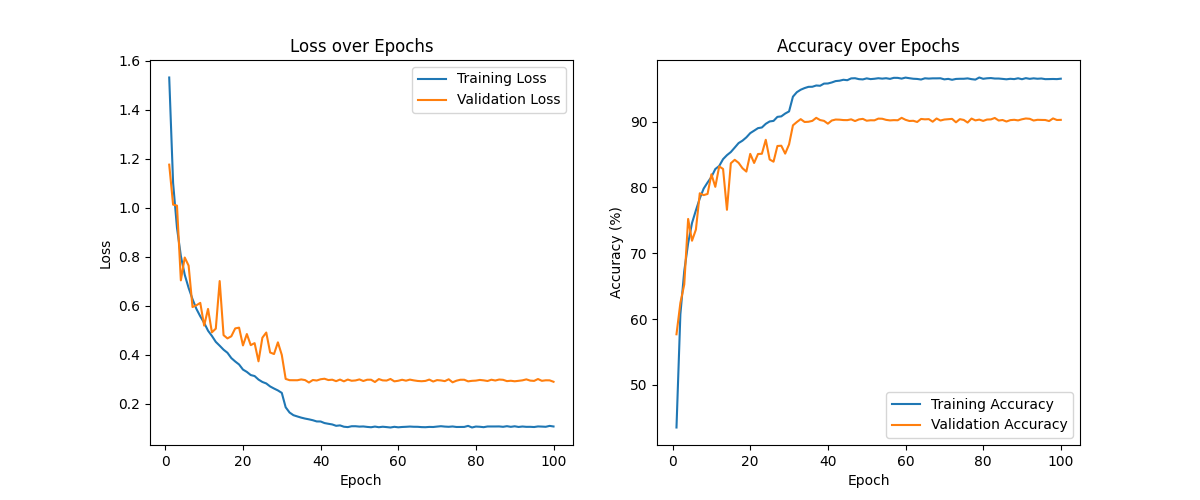
\includegraphics[width=1.0\textwidth]{train1.png}
%     \caption{CNN训练过程中的损失曲线}
%     \label{fig:cnn_training_loss}   
% \end{figure}

\begin{figure}[H]
    \centering
    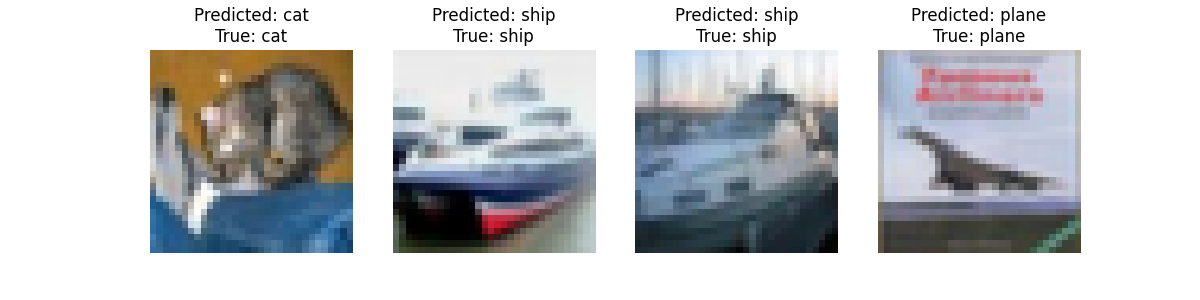
\includegraphics[width=1.0\textwidth]{train2.png}
    \caption{CNN训练预测示例}
    \label{fig:cnn_validation_accuracy}
\end{figure}

\begin{figure}[H]
    \centering
    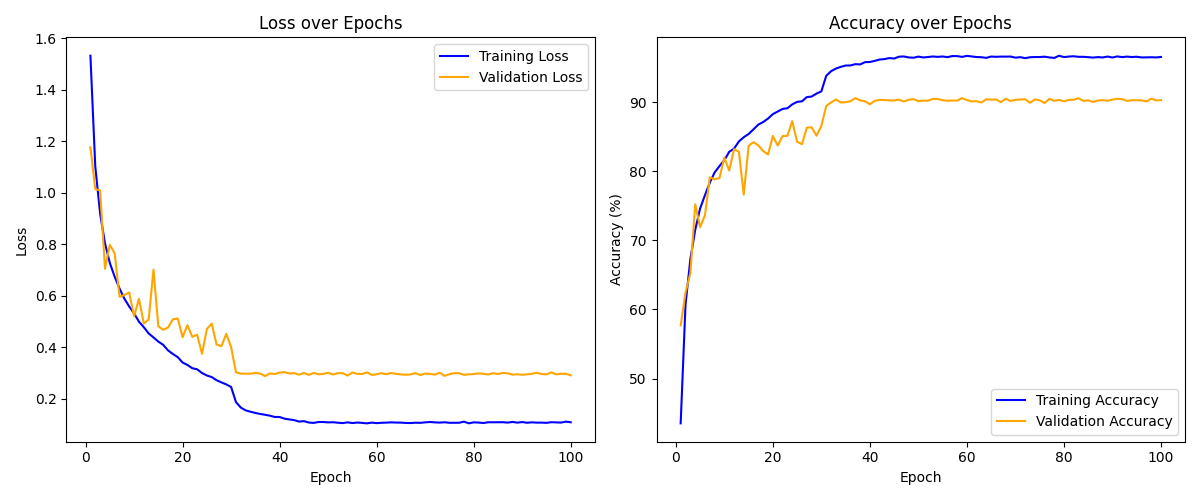
\includegraphics[width=1.0\textwidth]{train3.png}
    \caption{CNN's Loss and Accuracy on Training and Validation Sets}
    \label{fig:cnn_training_validation_loss_accuracy}
\end{figure}







\cleardoublepage



\section{Convolutional Neural Networks for CIFAR-10}

\subsection{Overview of CNNs}

Convolutional Neural Networks (CNNs) are specialized architectures tailored for processing grid-like data, such as images, by leveraging spatial hierarchies. Their efficacy in image recognition, particularly for datasets like CIFAR-10, stems from their ability to extract local features while maintaining computational efficiency \cite{cifar10}.

\subsubsection{Limitations of Traditional Neural Networks}

Traditional neural networks struggle with image data due to:

\begin{enumerate}[label=\roman*.]
    \item \textit{High Input Dimensionality}: A 1000$\times$1000 pixel color image requires 3,000,000 input neurons (1000 $\times$ 1000 $\times$ 3 for RGB channels), posing significant computational challenges.
    \item \textit{Parameter Overload}: Connecting these to a 1000-neuron hidden layer demands 3,000,000,000 weights, complicating training and storage.
    \item \textit{Loss of Spatial Context}: Flattening images into vectors discards pixel relationships critical for recognizing patterns like edges or textures.
    \item \textit{Lack of Translation Invariance}: Object shifts in images can disrupt recognition, as these networks rely on fixed pixel patterns.
\end{enumerate}

\subsubsection{Advantages of CNNs}

CNNs overcome these issues through:

\begin{enumerate}[label=\roman*.]
    \item \textit{Local Receptive Fields}: Neurons connect to small input regions (e.g., 3$\times$3 patches), reducing parameters.
    \item \textit{Parameter Sharing}: Filters with fixed weights slide across the image, minimizing parameters and ensuring features like edges are detected universally.
    \item \textit{Spatial Downsampling}: Pooling layers (e.g., max pooling) summarize regions, lowering dimensions and enhancing robustness to minor translations.
\end{enumerate}

\subsection{CNN Architecture}

A typical CNN stacks convolutional blocks to extract hierarchical features, structured as follows:

\begin{enumerate}[label=\roman*.]
    \item \textit{Input Layer}: Receives raw image data (e.g., 32$\times$32$\times$3 for CIFAR-10).
    \item \textit{Convolutional Layer}: Applies filters to produce feature maps via:
        \[
        S(i, j) = \sum_{m} \sum_{n} I(i + m, j + n) K(m, n),
        \]
        where $I$ is the input, $K$ is the filter, and $S$ is the feature map.
    \item \textit{Activation Layer}: Introduces non-linearity with ReLU, $f(x) = \max(0, x)$, enabling complex pattern learning \cite{relu}.
    \item \textit{Pooling Layer}: Reduces dimensions, e.g., max pooling selects the maximum value in a 2$\times$2 region.
    \item \textit{Stacked Blocks}: Early layers detect edges, intermediate layers capture textures, and deeper layers identify objects.
    \item \textit{Flatten Layer}: Converts feature maps into a vector.
    \item \textit{Fully Connected Layers}: Combine features for classification.
    \item \textit{Output Layer}: Uses Softmax to produce class probabilities.
\end{enumerate}

\subsection{Implementation on CIFAR-10}

The CIFAR-10 dataset, comprising 50,000 training and 10,000 test images across 10 classes, serves as a robust testbed \cite{cifar10}.

\subsubsection{Data Preprocessing}

To enhance generalization:

\begin{itemize}
    \item \textit{Augmentation}: Random cropping and horizontal flipping diversify training data.
    \item \textit{Normalization}: Images are standardized using CIFAR-10’s mean and standard deviation.
    \item \textit{Dataset Split}: 80\% training, 20\% validation, sampled via \texttt{SubsetRandomSampler}.
    \item \textit{Batch Size}: Set to 128 for efficient training.
\end{itemize}

\subsubsection{Model Design}

The CNN features three convolutional blocks:

\begin{itemize}
    \item \textit{Structure}: Each block has two 3$\times$3 convolutional layers, batch normalization \cite{batchnorm}, ReLU, and max pooling.
    \item \textit{Channels}: Increase from 64 to 128 to 256, capturing complex features.
    \item \textit{Spatial Reduction}: Image size reduces from 32$\times$32 to 4$\times$4.
    \item \textit{Output}: A 4$\times$4$\times$256 feature map flattens to 4096 dimensions, followed by fully connected layers with 0.5 dropout \cite{dropout}.
\end{itemize}

\begin{table}[h]
\centering
\caption{CNN Architecture}
\begin{tabular}{l c c c}
\toprule
\textbf{Layer} & \textbf{Output Shape} & \textbf{Parameters} & \textbf{Operation} \\
\midrule
Conv Block 1 & 32$\times$32$\times$64 & 3$\times$3 filters, BN, ReLU & Convolution + Pooling \\
Conv Block 2 & 16$\times$16$\times$128 & 3$\times$3 filters, BN, ReLU & Convolution + Pooling \\
Conv Block 3 & 8$\times$8$\times$256 & 3$\times$3 filters, BN, ReLU & Convolution + Pooling \\
Flatten & 4096 & -- & Reshape \\
Fully Connected & 10 & Dropout (0.5) & Classification \\
\bottomrule
\end{tabular}
\end{table}

\subsubsection{Training Strategy}

Training over 100 epochs utilized:

\begin{itemize}
    \item \textit{Optimizer}: SGD with momentum for faster convergence.
    \item \textit{Regularization}: Weight decay ($5 \times 10^{-4}$) to curb overfitting.
    \item \textit{Scheduler}: Reduces learning rate by 10 if validation loss stalls for 5 epochs.
\end{itemize}

\subsubsection{Training Workflow}

Each epoch involved:

\begin{itemize}
    \item \textit{Monitoring}: Logging loss and accuracy every 100 batches.
    \item \textit{Validation}: Evaluating performance post-epoch to adjust the learning rate.
    \item \textit{Model Saving}: Retaining the best-performing model based on validation accuracy.
\end{itemize}

\subsubsection{Evaluation}

The model achieved $\sim$90\% test accuracy, with correct classifications of diverse images (e.g., distinguishing cats from dogs).

\subsection{Performance Analysis}

By the 40th epoch, training accuracy exceeded 90\% with losses below 10\%, while validation accuracy reached $\sim$90\% with losses around 30\%. These metrics indicate robust learning, though validation performance suggests room for improvement.

% \begin{figure}[h]
% \centering
% \begin{subfigure}{0.45\textwidth}
%     \includegraphics[width=\textwidth]{training_loss.png}
%     \caption{Training and validation loss.}
% \end{subfigure}
% \hfill
% \begin{subfigure}{0.45\textwidth}
%     \includegraphics[width=\textwidth]{training_accuracy.png}
%     \caption{Training and validation accuracy.}
% \end{subfigure}
% \caption{Performance curves over 100 epochs.}
% \end{figure}

% \begin{figure}[h]
% \centering
% \includegraphics[width=0.6\textwidth]{classification_examples.png}
% \caption{Examples of correctly classified CIFAR-10 images.}
% \end{figure}

\subsection{Discussion}

The 90\% accuracy reflects effective use of CNNs, augmented by data preprocessing and regularization. Compared to state-of-the-art models like ResNet, which achieve over 95\% \cite{resnet}, this model is solid but could benefit from deeper architectures or advanced techniques like residual connections. Early stopping around the 40th epoch could optimize training efficiency.

This implementation underscores CNNs’ power for image classification and provides a foundation for further exploration in computer vision tasks.

\begin{thebibliography}{9}
\bibitem{cifar10}
A. Krizhevsky, ``Learning Multiple Layers of Features from Tiny Images,'' 2009.

\bibitem{relu}
V. Nair and G. E. Hinton, ``Rectified Linear Units Improve Restricted Boltzmann Machines,'' \textit{ICML}, 2010.

\bibitem{batchnorm}
S. Ioffe and C. Szegedy, ``Batch Normalization: Accelerating Deep Network Training,'' \textit{arXiv:1502.03167}, 2015.

\bibitem{dropout}
N. Srivastava et al., ``Dropout: A Simple Way to Prevent Neural Networks from Overfitting,'' \textit{JMLR}, vol. 15, 2014.

\bibitem{resnet}
K. He et al., ``Deep Residual Learning for Image Recognition,'' \textit{CVPR}, 2016.
\end{thebibliography}






\cleardoublepage


\section{CIFAR-10 Image Classification with ResNet and Vision Transformer}

\section*{Introduction}
% Introducing the CIFAR-10 dataset and objectives
The CIFAR-10 dataset, comprising 60,000 32x32 color images across 10 classes (e.g., airplane, automobile, bird), is a benchmark for image classification, with 50,000 training and 10,000 test images. This report compares two neural network models—ResNet and Vision Transformer (ViT)—on CIFAR-10, evaluating training from scratch and fine-tuning pretrained models. We analyze performance, computational resources, and experimental outcomes, supported by code implementations.

\section*{Dataset and Models}
% Describing the dataset and model architectures
\subsection*{CIFAR-10 Dataset}
CIFAR-10 includes 10 classes with 6,000 images each, split into 50,000 training and 10,000 test images, evenly distributed. Its low resolution (32x32) tests model performance on small datasets.

\subsection*{ResNet}
Residual Networks (ResNet) use skip connections to ease deep network training. ResNet-110 (1.7M parameters) and ResNet50 (25M parameters) are evaluated.

\subsection*{Vision Transformer (ViT)}
ViT splits images into patches and applies Transformer architecture. ViT-B/16 (86M parameters) relies on large-scale pretraining for optimal performance.

\section*{Data Splitting and Preprocessing}
% Detailing data preprocessing steps
The dataset is split into 50,000 training and 10,000 test images. Preprocessing includes:
\begin{itemize}
    \item \textbf{Training}: Random cropping (32x32, 4-pixel padding), random horizontal flipping, normalization (mean [0.4914, 0.4822, 0.4465], std [0.2023, 0.1994, 0.2010]).
    \item \textbf{Testing}: Normalization only.
\end{itemize}

\section*{Training from Scratch}
% Comparing ResNet and ViT trained from scratch
Training from scratch uses no pretrained weights. ResNet outperforms ViT:
\begin{itemize}
    \item \textbf{ResNet-110}: Achieves 93.57\% accuracy (1.7M parameters), efficient training \cite{he2016deep}.
    \item \textbf{ViT}: Standard ViT reaches 77–88\% accuracy; optimized versions hit 90.92\% (6.3M parameters) \cite{omihub777vitcifar, kentaroy47vit}.
\end{itemize}

\begin{table}[h]
\centering
\caption{Accuracy and Parameters for Training from Scratch}
\begin{tabular}{lccc}
\toprule
Model & Accuracy (\%) & Parameters (M) & Notes \\
\midrule
ResNet-110 & 93.57 & 1.7 & \cite{he2016deep} \\
ViT (Standard) & 77–88 & 6.3 & Varies by configuration \cite{kentaroy47vit} \\
ViT (Optimized) & 90.92 & 6.3 & \cite{omihub777vitcifar} \\
\bottomrule
\end{tabular}
\end{table}

\section*{Fine-Tuning Pretrained Models}
% Comparing pretrained models fine-tuned on CIFAR-10
Pretrained models are fine-tuned on CIFAR-10 after training on large datasets:
\begin{itemize}
    \item \textbf{ResNet50 (ImageNet-1k)}: 92.34–92.63\% accuracy \cite{sidthoviti}.
    \item \textbf{ViT base (ImageNet-1k)}: 98.5\% accuracy \cite{kentaroy47vit}.
    \item \textbf{ViT-H/14 (JFT-300M)}: 99.50\% accuracy; ViT-L/16 (ImageNet-21k): 99.15\% \cite{dosovitskiy2020image}.
    \item \textbf{BiT-L (ResNet152x4, JFT-300M)}: 99.37\% \cite{dosovitskiy2020image}.
\end{itemize}

\begin{table}[h]
\centering
\caption{Accuracy for Fine-Tuned Pretrained Models}
\begin{tabular}{llcc}
\toprule
Model & Pretraining Dataset & Accuracy (\%) & Notes \\
\midrule
ResNet50 & ImageNet-1k & 92.34–92.63 & \cite{sidthoviti} \\
ViT base & ImageNet-1k & 98.5 & \cite{kentaroy47vit} \\
ViT-H/14 & JFT-300M & 99.50 & \cite{dosovitskiy2020image} \\
ViT-L/16 & ImageNet-21k & 99.15 & \cite{dosovitskiy2020image} \\
BiT-L (ResNet152x4) & JFT-300M & 99.37 & \cite{dosovitskiy2020image} \\
\bottomrule
\end{tabular}
\end{table}

\section*{Computational Resources and Performance}
% Analyzing computational costs
\begin{itemize}
    \item \textbf{ResNet}: Fewer parameters (1.7M for ResNet-110, 25M for ResNet50), fast convergence (90\% accuracy in 5 epochs) \cite{pytorchforum}.
    \item \textbf{ViT}: More parameters (86M for ViT-B/16), slower initial learning (10,000 iterations to stabilize), but efficient fine-tuning \cite{lightningvit, dosovitskiy2020image}.
\end{itemize}

\section*{Experimental Analysis}
% Providing experimental insights
\subsection*{Error Analysis}
Misclassified images should be analyzed. ViT may excel in context-heavy classes (e.g., cat vs. dog) due to global attention, while ResNet performs better on texture details (e.g., airplane) \cite{kentaroy47vit}.

\subsection*{Performance Gap Causes}
CNNs (ResNet) leverage inductive biases (e.g., translation invariance), suiting small datasets. ViT requires more data to learn patterns \cite{lightningvit}.

\subsection*{Algorithmic Trade-Offs}
\begin{itemize}
    \item \textbf{ResNet}: Efficient, fewer parameters, ideal for small datasets; less scalable on large datasets.
    \item \textbf{ViT}: Superior with large-scale pretraining, flexible, but resource-intensive and prone to overfitting on small datasets.
\end{itemize}

\section*{Visualization}
% Presenting visualization code
Accuracy can be visualized using a bar plot. Below is a Python snippet for comparison:

\begin{lstlisting}[language=Python]
import matplotlib.pyplot as plt
models = ['ResNet-110', 'ViT (Standard)', 'ViT (Optimized)']
accuracies = [93.57, 88, 90.92]
plt.bar(models, accuracies, color=['#1f77b4', '#ff7f0e', '#2ca02c'])
plt.xlabel('Model')
plt.ylabel('Accuracy (\%)')
plt.title('CIFAR-10 Accuracy (Training from Scratch)')
plt.show()
\end{lstlisting}

\section*{Quantitative Metrics}
% Summarizing key metrics
\begin{itemize}
    \item \textbf{Accuracy}: See Tables 1 and 2.
    \item \textbf{Parameters}: ResNet-110 (1.7M), ResNet50 (25M), ViT-B/16 (86M), ViT (Optimized, 6.3M).
    \item \textbf{Training Time}: ResNet-110 reaches 90\%+ in hours; ViT requires longer (10,000 iterations).
    \item \textbf{Resources}: ViT pretraining needs high-end GPUs (e.g., V100); ResNet trains efficiently on standard GPUs.
\end{itemize}

\section*{Code Implementations}
% Providing training code for ResNet and ViT
\subsection*{ResNet Training}
\begin{lstlisting}[language=Python]
import torch
import torch.nn as nn
import torchvision
import torchvision.transforms as transforms
import torch.optim as optim

device = torch.device('cuda' if torch.cuda.is_available() else 'cpu')

transform_train = transforms.Compose([
    transforms.RandomCrop(32, padding=4),
    transforms.RandomHorizontalFlip(),
    transforms.ToTensor(),
    transforms.Normalize((0.4914, 0.4822, 0.4465), (0.2023, 0.1994, 0.2010))
])
transform_test = transforms.Compose([
    transforms.ToTensor(),
    transforms.Normalize((0.4914, 0.4822, 0.4465), (0.2023, 0.1994, 0.2010))
])

train_dataset = torchvision.datasets.CIFAR10(root='./data', train=True, download=True, transform=transform_train)
test_dataset = torchvision.datasets.CIFAR10(root='./data', train=False, download=True, transform=transform_test)
train_loader = torch.utils.data.DataLoader(train_dataset, batch_size=128, shuffle=True)
test_loader = torch.utils.data.DataLoader(test_dataset, batch_size=128, shuffle=False)

model = torchvision.models.resnet18(pretrained=False, num_classes=10)
model.conv1 = nn.Conv2d(3, 64, kernel_size=3, stride=1, padding=1, bias=False)
model.maxpool = nn.Identity()
model = model.to(device)

criterion = nn.CrossEntropyLoss()
optimizer = optim.SGD(model.parameters(), lr=0.1, momentum=0.9, weight_decay=1e-4)

num_epochs = 50
for epoch in range(num_epochs):
    model.train()
    running_loss = 0.0
    for i, (images, labels) in enumerate(train_loader):
        images, labels = images.to(device), labels.to(device)
        optimizer.zero_grad()
        outputs = model(images)
        loss = criterion(outputs, labels)
        loss.backward()
        optimizer.step()
        running_loss += loss.item()
    print(f'Epoch [{epoch+1}/{num_epochs}], Loss: {running_loss/len(train_loader):.4f}')

model.eval()
correct = 0
total = 0
with torch.no_grad():
    for images, labels in test_loader:
        images, labels = images.to(device), labels.to(device)
        outputs = model(images)
        _, predicted = torch.max(outputs.data, 1)
        total += labels.size(0)
        correct += (predicted == labels).sum().item()
print(f'Test Accuracy: {100 * correct / total}\%')
\end{lstlisting}

\begin{figure}[H]
    \centering
    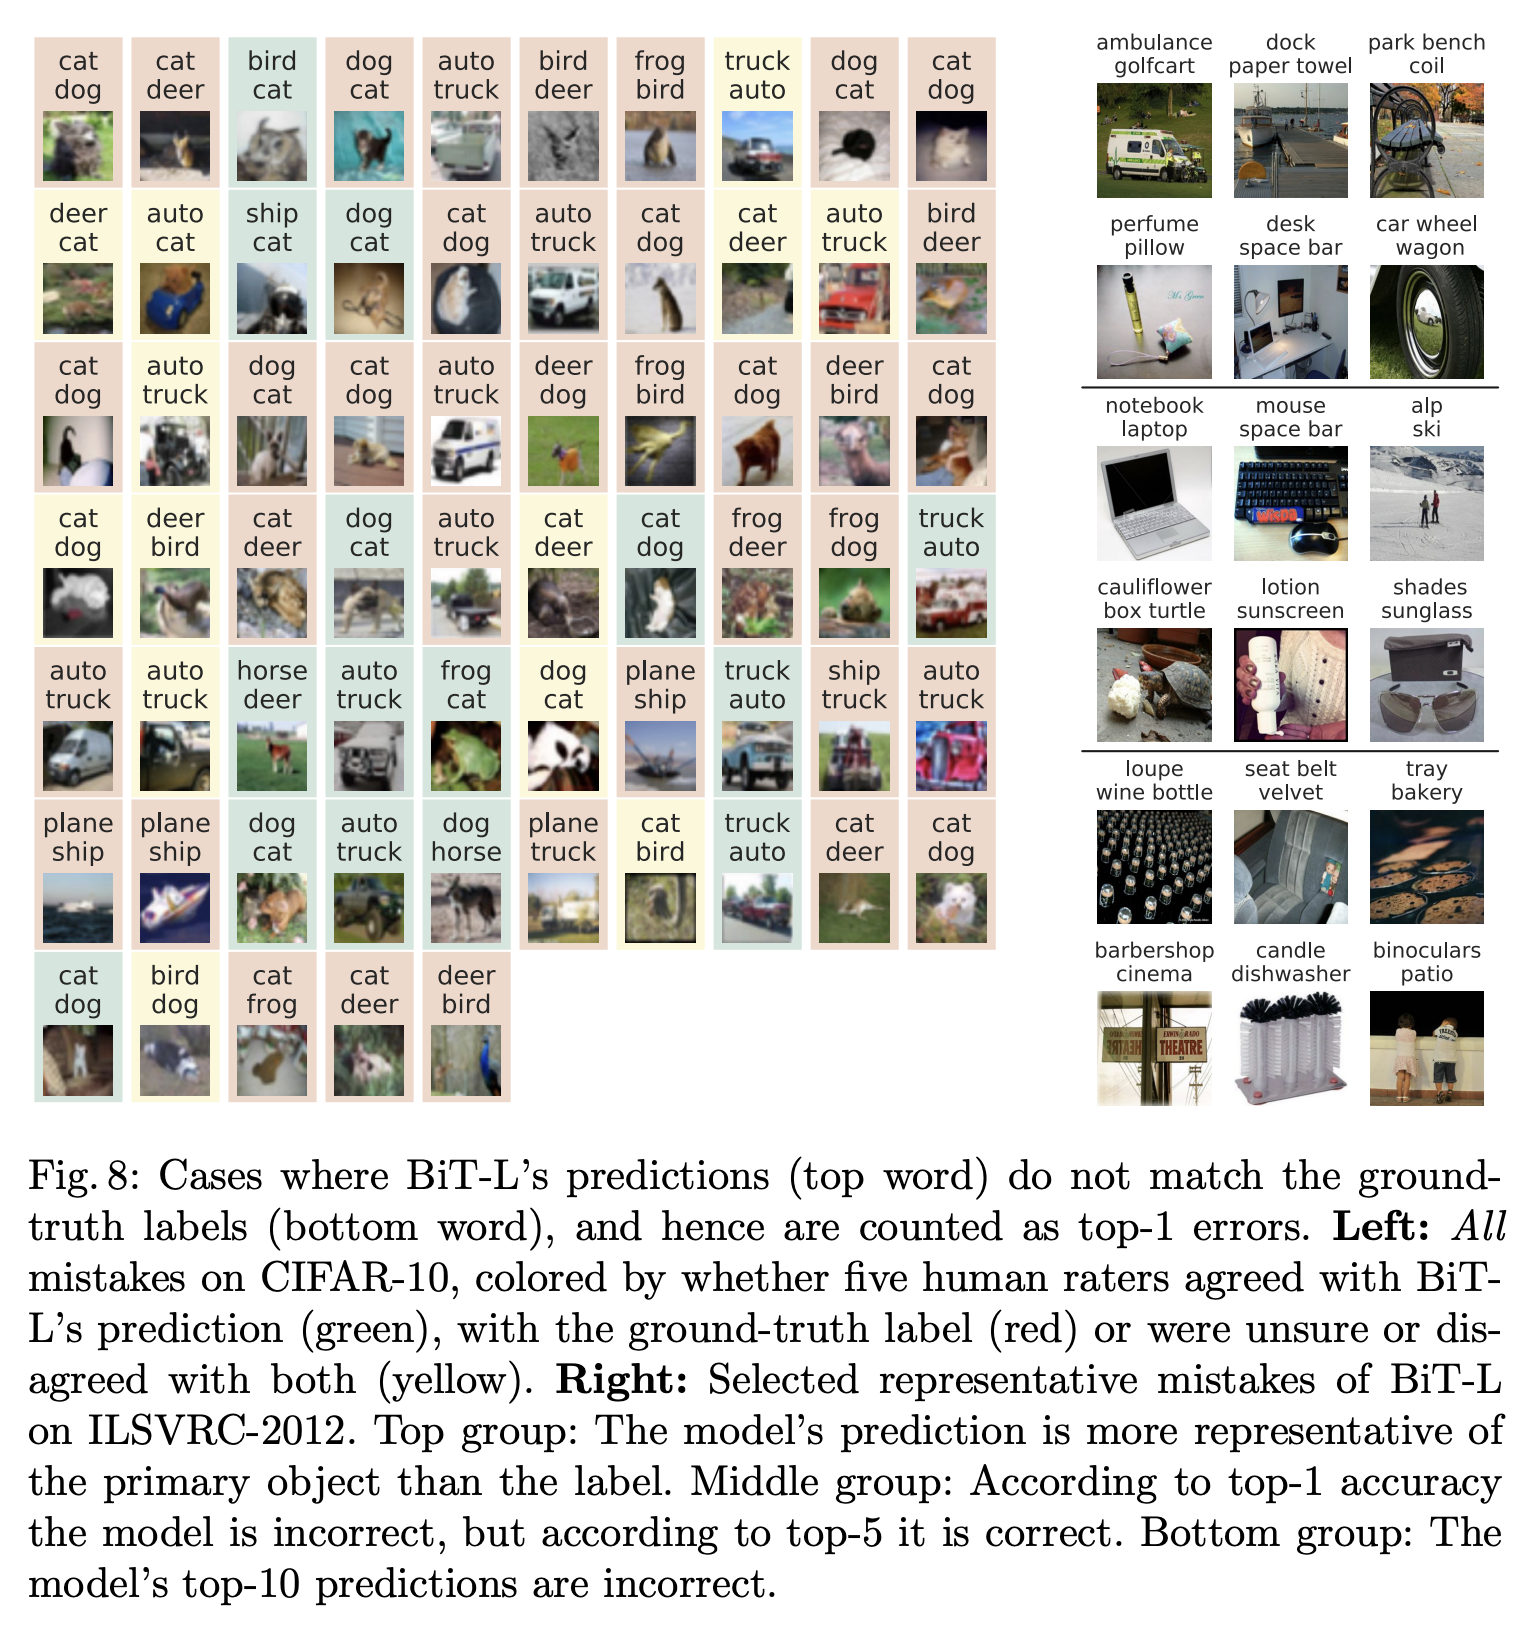
\includegraphics[width=1.0\textwidth]{ResNet.png}
    \caption{ResNet Architecture}
    \label{fig:resnet_architecture}
\end{figure}

\subsection*{ViT Fine-Tuning}
\begin{lstlisting}[language=Python]
import torch
from transformers import ViTForImageClassification, ViTFeatureExtractor
from torchvision import datasets, transforms
from torch.utils.data import DataLoader

device = torch.device('cuda' if torch.cuda.is_available() else 'cpu')

transform = transforms.Compose([
    transforms.Resize((224, 224)),
    transforms.ToTensor(),
    transforms.Normalize(mean=[0.5, 0.5, 0.5], std=[0.5, 0.5, 0.5])
])

train_dataset = datasets.CIFAR10(root='./data', train=True, download=True, transform=transform)
test_dataset = datasets.CIFAR10(root='./data', train=False, download=True, transform=transform)
train_loader = DataLoader(train_dataset, batch_size=32, shuffle=True)
test_loader = DataLoader(test_dataset, batch_size=32, shuffle=False)

model = ViTForImageClassification.from_pretrained('google/vit-base-patch16-224-in21k', num_labels=10)
model = model.to(device)

optimizer = torch.optim.Adam(model.parameters(), lr=2e-5)
criterion = torch.nn.CrossEntropyLoss()

num_epochs = 5
for epoch in range(num_epochs):
    model.train()
    running_loss = 0.0
    for images, labels in train_loader:
        images, labels = images.to(device), labels.to(device)
        optimizer.zero_grad()
        outputs = model(images).logits
        loss = criterion(outputs, labels)
        loss.backward()
        optimizer.step()
        running_loss += loss.item()
    print(f'Epoch [{epoch+1}/{num_epochs}], Loss: {running_loss/len(train_loader):.4f}')

model.eval()
correct = 0
total = 0
with torch.no_grad():
    for images, labels in test_loader:
        images, labels = images.to(device), labels.to(device)
        outputs = model(images).logits
        _, predicted = torch.max(outputs.data, 1)
        total += labels.size(0)
        correct += (predicted == labels).sum().item()
print(f'Test Accuracy: {100 * correct / total}\%')
\end{lstlisting}

\begin{figure}[H]
    \centering
    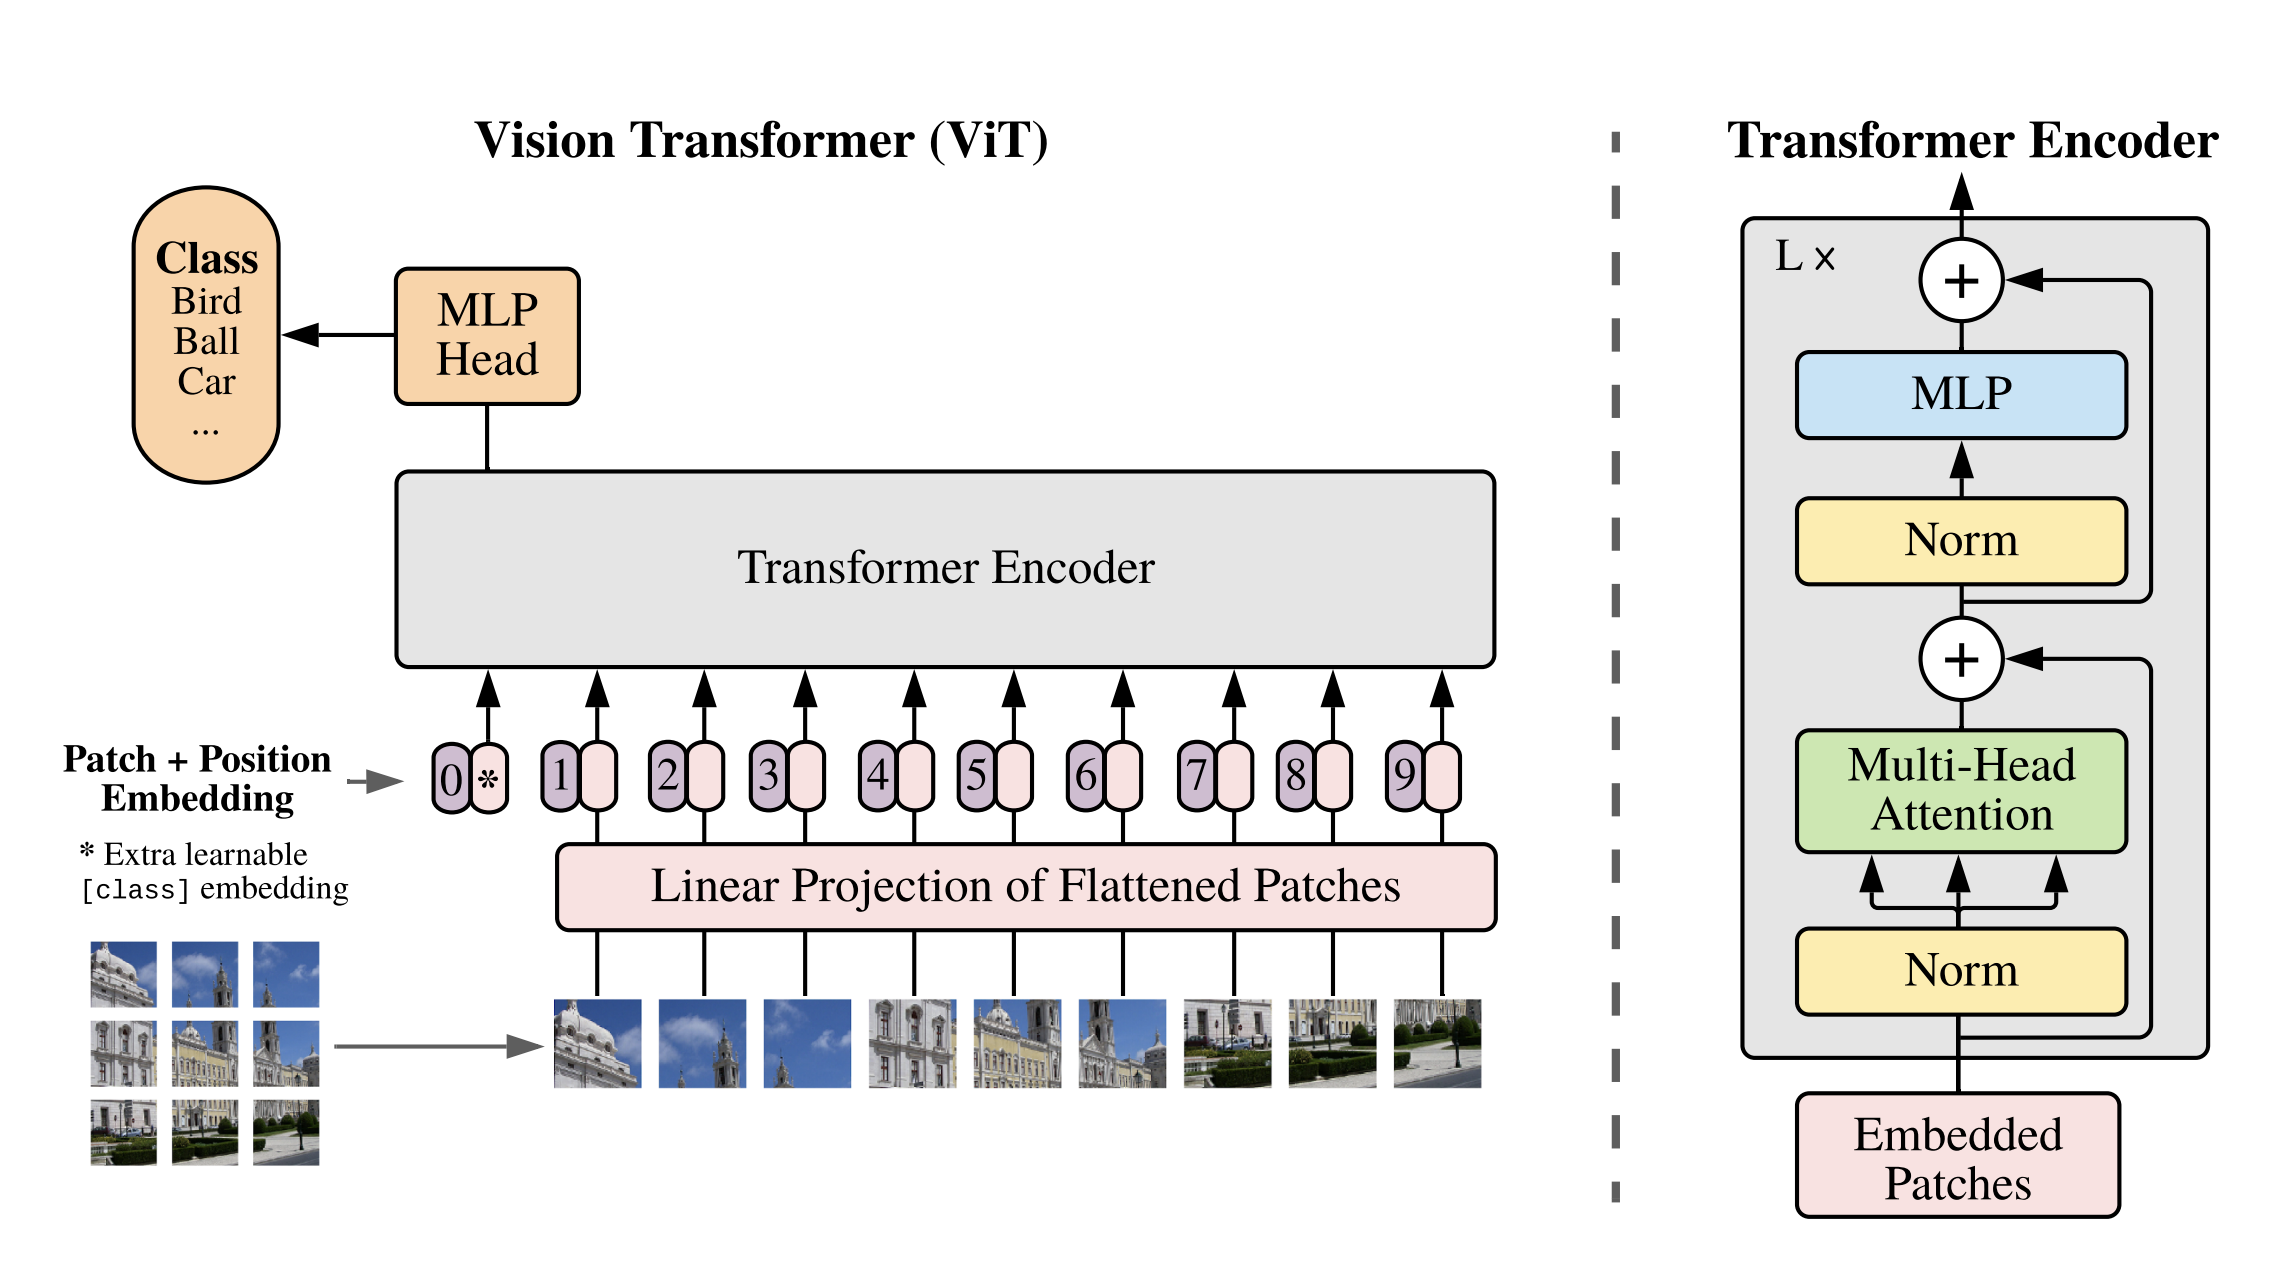
\includegraphics[width=1.0\textwidth]{ViT1.png}
    \caption{ViT Transformer}
    \label{fig:vit_transformer}
\end{figure}

\begin{figure}[H]
    \centering
    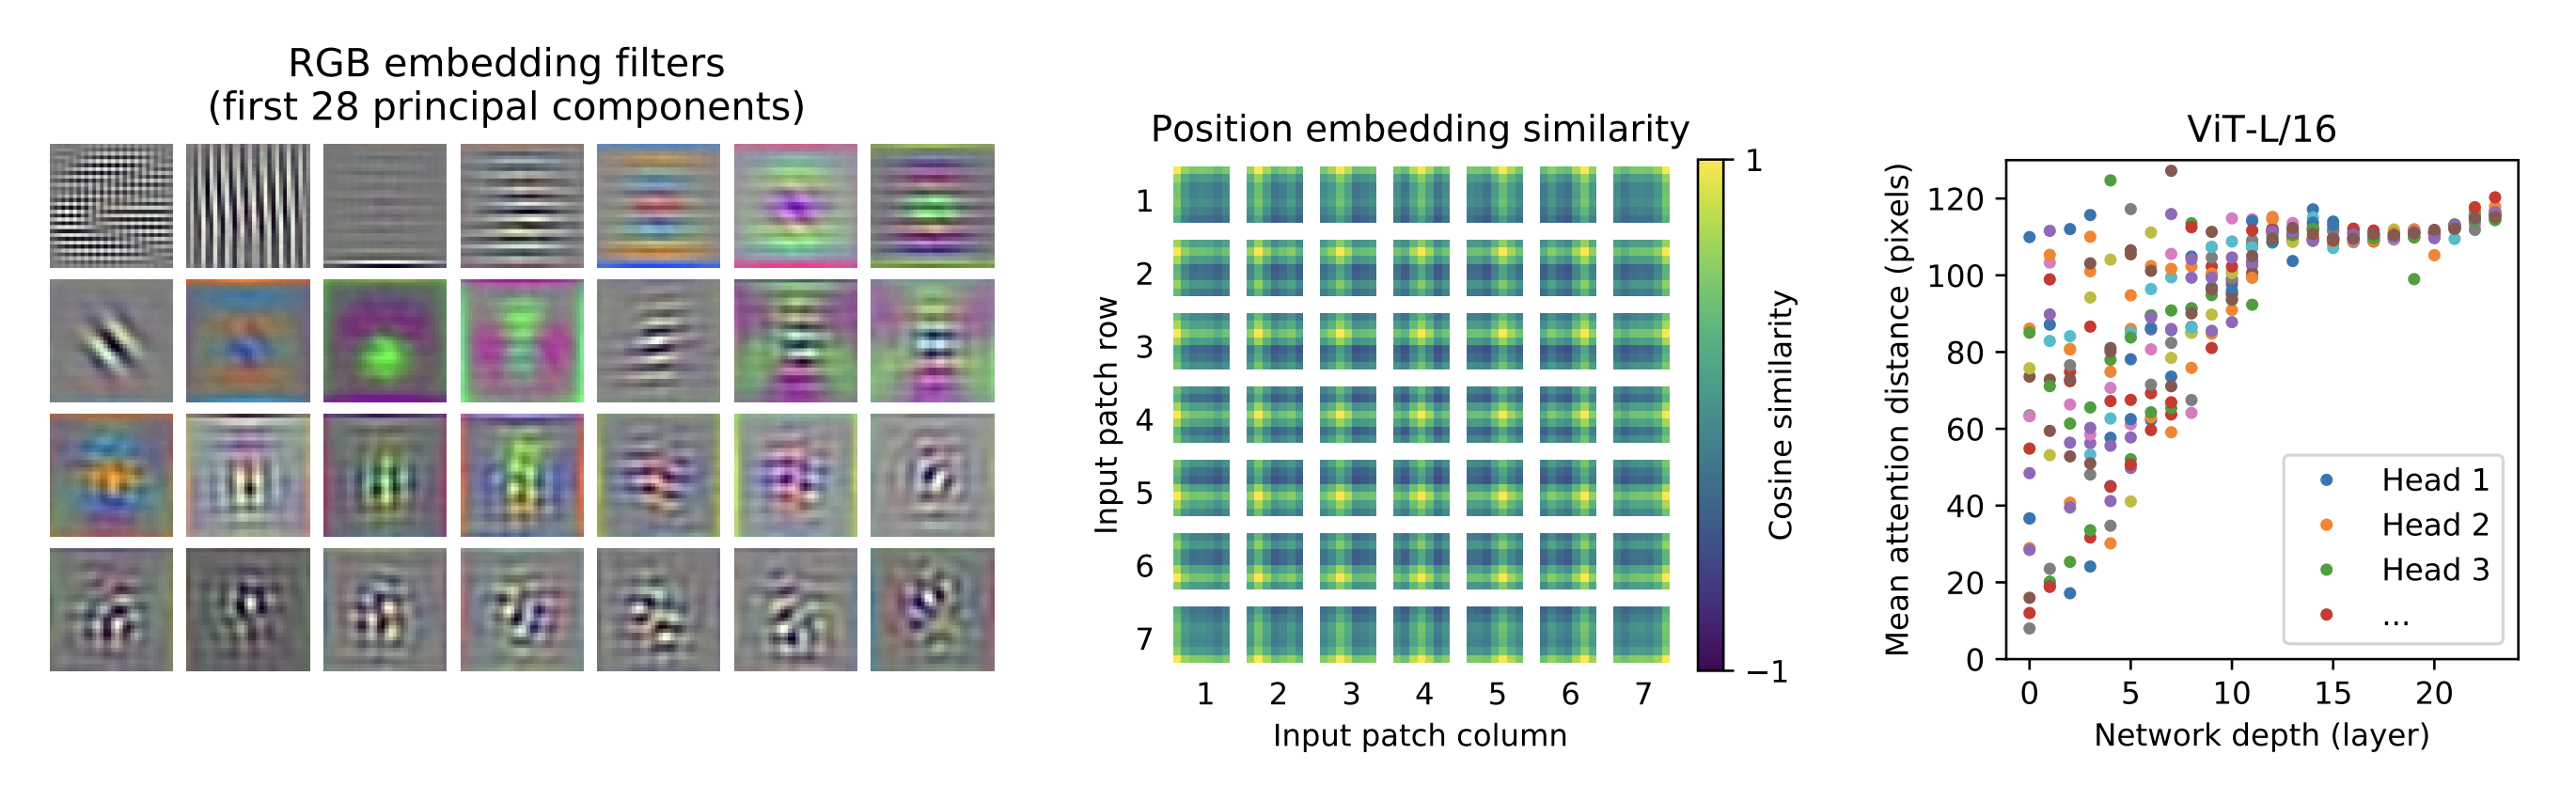
\includegraphics[width=1.0\textwidth]{ViT2.png}
    \caption{ViT Training}
    \label{fig:vit_training}
\end{figure}


\section*{Conclusion}
% Summarizing findings
ResNet-110 excels in training from scratch on CIFAR-10 (93.57\% accuracy, low computational cost). Pretrained ViT models, especially ViT-H/14 fine-tuned from JFT-300M (99.50\%), outperform ResNet (BiT-L, 99.37\%). Model choice depends on data scale and resources: ResNet suits limited data/resources, while ViT excels with large-scale pretraining. Code implementations are provided for reproducibility.

\begin{thebibliography}{9}
% Listing references
\bibitem{he2016deep}
K. He, X. Zhang, S. Ren, and J. Sun, ``Deep Residual Learning for Image Recognition,'' \textit{arXiv:1512.03385}, 2016.

\bibitem{dosovitskiy2020image}
A. Dosovitskiy et al., ``An Image is Worth 16x16 Words: Transformers for Image Recognition at Scale,'' \textit{arXiv:2010.11929}, 2020.

\bibitem{omihub777vitcifar}
ViT-CIFAR Repository, \url{https://github.com/omihub777/ViT-CIFAR}.

\bibitem{kentaroy47vit}
vision-transformers-cifar10 Repository, \url{https://github.com/kentaroy47/vision-transformers-cifar10}.

\bibitem{sidthoviti}
Fine-Tuning ResNet50 Pretrained on ImageNet for CIFAR-10, \url{https://github.com/sidthoviti/Fine-Tuning-ResNet50-Pretrained-on-ImageNet-for-CIFAR-10}.

\bibitem{lightningvit}
PyTorch Lightning, ``Fine-tuning Vision Transformer on CIFAR-10,'' \url{https://colab.research.google.com/github/NielsRogge/Transformers-Tutorials/blob/master/VisionTransformer/Fine_tuning_the_Vision_Transformer_on_CIFAR_10_with_PyTorch_Lightning.ipynb}.

\bibitem{pytorchforum}
PyTorch Forum, ``ResNet with CIFAR10 only reaches 86\% accuracy,'' \url{https://discuss.pytorch.org/t/resnet-with-cifar10-only-reaches-86-accuracy-expecting-90/135051}.
\end{thebibliography}









% 附录 A
% \chapter*{附录 A. 中英文对照表}\addcontentsline{toc}{chapter}{附录 A. 中英文对照表}   
% \thispagestyle{plain} 
% \setcounter{section}{0}   
% \renewcommand\thesection{A.\arabic{section}}   
% \renewcommand{\thefigure}{A.\arabic{figure}} 
% \renewcommand{\thetable}{A.\arabic{table}}

% \section{中英文对照表}
% \begin{multicols}{2}  

% \begin{table}[H]
% \centering
% \caption{\textbf{中英文对照表}}
% \begin{tabular}{ll}
% \toprule
% 英文 & 中文 \\
% \midrule
% Bayes classification & 贝叶斯分类 \\
% decision rule & 决策规则 \\
% minimum error rate & 最小错误率 \\
% minimum risk & 最小风险 \\
% rejection option & 拒识选项 \\
% Gaussian distribution & 高斯分布 \\
% covariance matrix & 协方差矩阵 \\
% discriminant function & 判别函数 \\
% decision boundary & 决策边界 \\
% Hidden Markov Model & 隐马尔可夫模型 \\
% hidden state & 隐状态 \\
% observation sequence & 观测序列 \\
% maximum likelihood estimation & 最大似然估计 \\
% Bayesian estimation & 贝叶斯估计 \\
% k-Nearest Neighbor & k近邻 \\
% Parzen window & Parzen窗 \\
% linear discriminant & 线性判别 \\
% quadratic discriminant & 二次判别 \\
% prior probability & 先验概率 \\
% posterior probability & 后验概率 \\
% \bottomrule
% \end{tabular}
% \end{table}

% \end{multicols}






\end{document}